We ran an in-memory adaptive simulation of a solderball array subject to thermal
creep~\cite{albanyThermalCreep}.
Fig.~\ref{fig:alb-adapt} depicts the results of the parallel adaptive analysis
using the in-memory integration of SPR and the PUMI
unstructured mesh tools with Albany.
The adaptive workflow ran four solve-adapt cycles on 256, 512, and 1024 cores of
an IBM Blue Gene/Q using an initial mesh of 8M tetrahedral elements.
Like the PHASTA adaptive test, the adapted meshes contain only
negligible differences across the range of core counts.

\begin{figure} \centering
  \includegraphics[width=0.49\textwidth]{results/albany/8M_9_adapt_eb.075/figs/t2-crinkle-zoom.eps}
  \includegraphics[width=0.49\textwidth]{results/albany/8M_9_adapt_eb.075/figs/t3-crinkle-zoom.eps}
  \includegraphics[width=0.49\textwidth]{results/albany/8M_9_adapt_eb.075/figs/t4-crinkle-zoom.eps}
  \includegraphics[width=0.49\textwidth]{results/albany/8M_9_adapt_eb.075/figs/t5-crinkle-zoom.eps}
  \caption[Four adaptation cycles of 3x3 solderball mesh.]{
    Four adaptation cycles (top to bottom, left to right) of 3x3 solderball
    mesh.
    The mesh is refined near the high stress gradients at the interface between
    the solderballs and the upper and lower slabs.
  }
  \label{fig:alb-adapt}
\end{figure}

Algorithm~\ref{alg:albanyAdapt} lists the steps of the Albany-PUMI adaptive
workflow.
The workflow begins by loading the PUMI mesh, geometric model, and XML formatted
problem definition ($l.$\ref{alg:albAdpLoadMesh}-\ref{alg:albAdpLoadXML}),
and then creating the node and element mesh connectivity
($l.$\ref{alg:albAdpConn}) and sets of mesh
entities with boundary conditions ($l.$\ref{alg:albAdpSets}) for Albany.
The PUMI mesh is kept in memory as the workflow enters into the solve-adapt
cycle ($l.$\ref{alg:albAdpWhile}).
At the top of the cycle one load step is solved ($l.$\ref{alg:albAdpSolve}).
Following the load step, the solution information (a displacement vector at
mesh nodes) and history-dependent state variables at integration points are
passed in-memory to an APF
\texttt{FieldShape}~\cite{ibanez2016pumi} ($l.$\ref{alg:albAdpGetFields}).
SPR then computes mesh-entity level error estimates based on an
improved Cauchy stress field ($l.$\ref{alg:albAdpSpr}).
The estimated error is then transformed into an isotropic mesh size field, which
MeshAdapt then uses to drive local mesh
modification procedures ($l.$\ref{alg:albAdpAdapt}).
As the mesh modifications (split, collapse, etc...) are applied the
\texttt{FieldShape} transfer operators~\cite{radovitzky1999,ortiz1991}
are called to determine the value of state variables at repositioned or newly
created integration points.
Between coarsening and refinement adaptation stages, Zoltan's
interface~\cite{devine2002zoltan} to ParMETIS is called to predictively balance
the mesh and prevent memory exhaustion on parts where heavy refinement occurs.
Once adaptation is complete ParMA rebalances the mesh
($l.$\ref{alg:albAdpParma}) to reduce element and vertex imbalances for improved
linear system assembly and solve performance.
The adaptive cycle concludes with the transformation of PUMI
unstructured mesh information ($l.$\ref{alg:albAdpConn2}-\ref{alg:albAdpSets2})
and APF field information ($l.$\ref{alg:albAdpSetFields}) into Albany analysis
data structures.

\begin{algorithm}
  \caption{Albany-PUMI Adaptive Loop}\label{alg:albanyAdapt}
  \small
  \begin{algorithmic}[1]
    \Procedure{adaptiveLoop}{$max\_steps$}
      \State $pumi\_mesh \gets$ load the partitioned PUMI mesh from
      disk\label{alg:albAdpLoadMesh}
      \State $geom \gets$ load the geometric model from disk
      \State $probdef \gets$ load the Albany problem definition from
      disk\label{alg:albAdpLoadXML}
      \State \Call{createConnectivity}{$pumi\_mesh$}\label{alg:albAdpConn} 
      \State \Call{createNodeAndSideSets}{$pumi\_mesh$,$probdef$}\label{alg:albAdpSets}
      \State $step\_number \gets$ 0
      \While{$step\_number < max\_steps$}\label{alg:albAdpWhile}
        \State \Call{solveLoadStep}{$step\_number$++}\label{alg:albAdpSolve}
        \State \Call{getFields}{$pumi\_mesh$}\label{alg:albAdpGetFields}
        \State $size\_field \gets$ \Call{SPR}{$pumi\_mesh$}\label{alg:albAdpSpr}
        \State \Call{MeshAdapt}{$pumi\_mesh$,$size\_field$}\label{alg:albAdpAdapt}
        \State \Call{ParMA}{vtx$>$elm,$pumi\_mesh$}\label{alg:albAdpParma}
        \State \Call{createConnectivity}{$pumi\_mesh$}\label{alg:albAdpConn2}
        \State \Call{createNodeAndSideSets}{$pumi\_mesh$,$probdef$}\label{alg:albAdpSets2} 
        \State \Call{setFields}{$pumi\_mesh$}\label{alg:albAdpSetFields}
      \EndWhile
    \EndProcedure
  \end{algorithmic}
\end{algorithm}

Fig.~\ref{fig:inmem-alb} depicts the factor of two performance advantage of
in-memory transfers of fields and mesh data between Albany,
PUMI, and SPR versus
the writing of the mesh to POSIX files.
Based on this data we estimate the performance advantage of the in-memory
approach over a file-based loop that both reads and writes files to be
about four times higher.
Another advantage demonstrated by this data is the low in-memory transfer time
imbalance; defined as maximum cycle time divided by the average cycle time.
The in-memory approach has less than a 6\% imbalance across all core counts
while the file writing approach has a 22\% imbalance at 512 cores (as shown by
the large error bar in Fig.~\ref{fig:inmem-alb}).
Since the heaviest parts in our test meshes have at most 5\% more elements and
12\% more vertices than the average part, and the data transfers are
proportional to the number of mesh vertices and elements on each part, then we
conclude that the observed imbalance in file-based I/O is attributable to
shared filesystem resource contention.

\begin{figure} \centering
  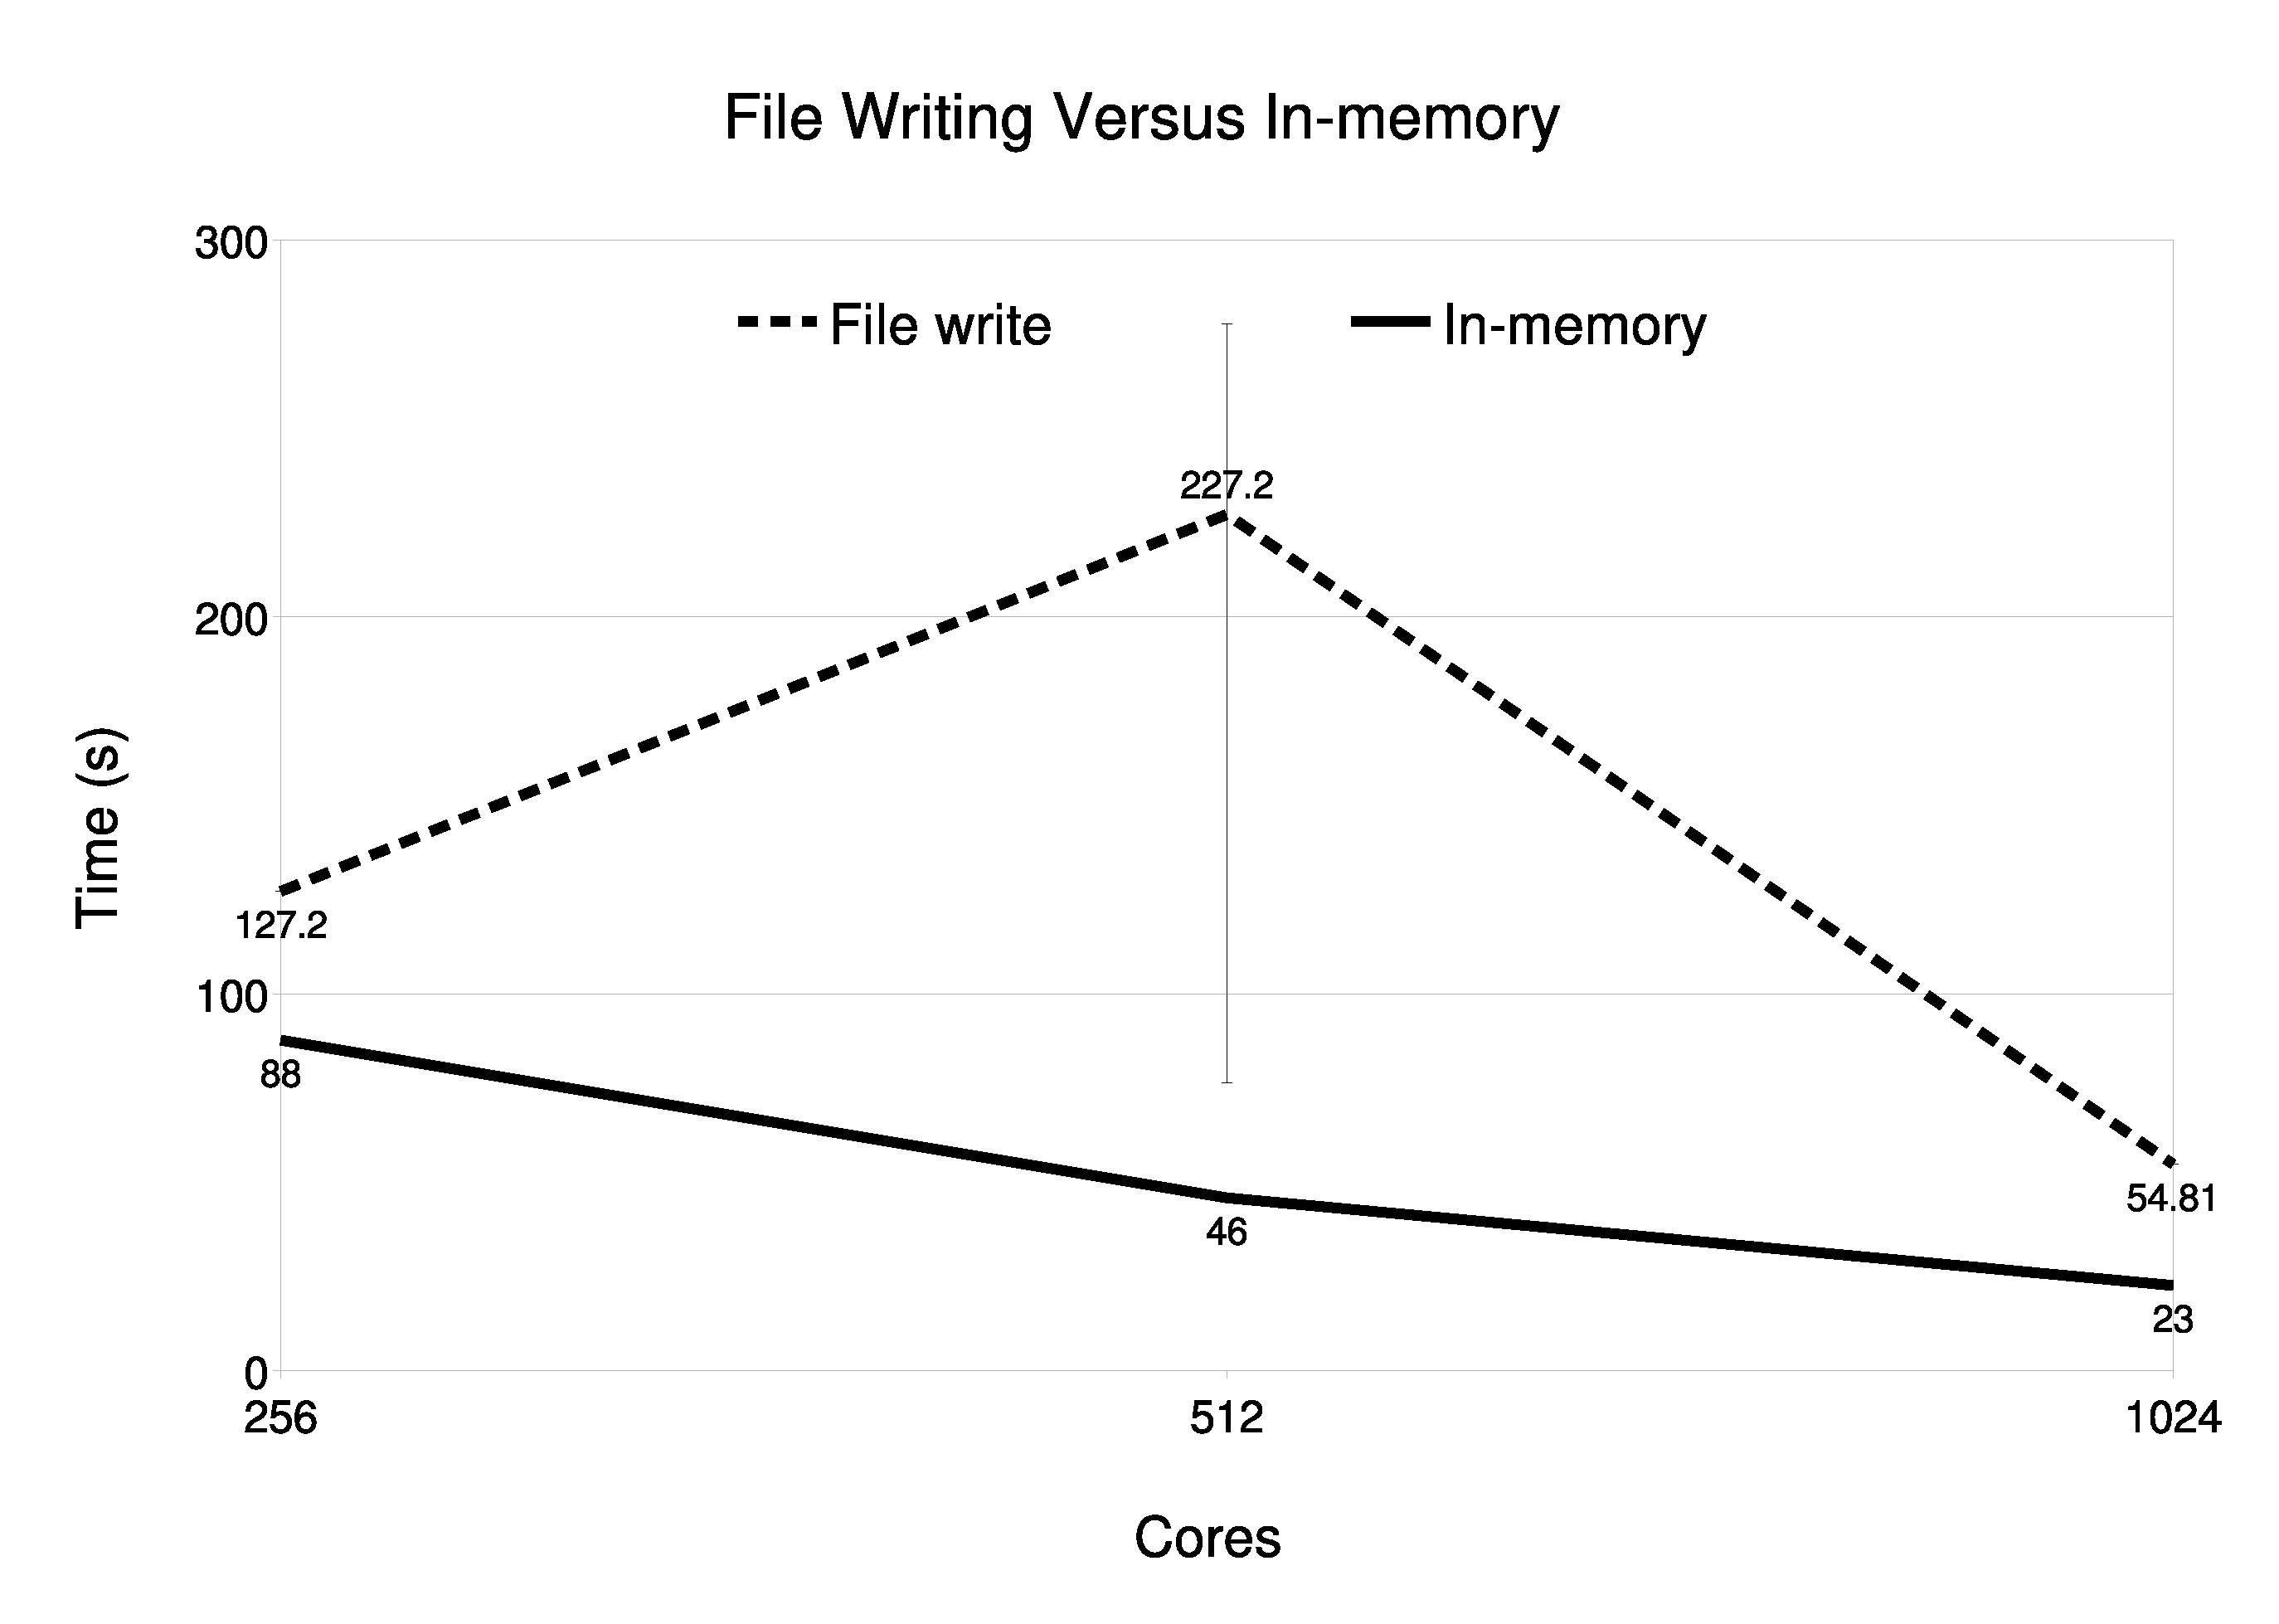
\includegraphics[width=.7\textwidth]{results/albany/compare.eps}
  \caption{
    Average per cycle file writing and in-memory transfer times.  Minimum and
    maximum bars are only shown for the 512 core file writing data point where
    they are 6\% more, or less, than the mean, respectively. Lower is better.}
  \label{fig:inmem-alb}
\end{figure}

Using the Albany-PUMI workflow we also simulated the tensile loading of the 2014
RPI Formula Hybrid race car suspension upright.
Fig.~\ref{fig:alb-upright} depicts the
upright in its initial state, and after multiple load steps.
Without adaptation the severe stretching of domain would result in invalid
elements and the subsequent failure of the analysis.

\begin{figure} \centering
  \includegraphics[width=.49\textwidth]{figures/upright/upright-initial.png}
  \includegraphics[width=.49\textwidth]{figures/upright/upright-final.png}
  \caption{
    Large deformation of the RPI Formula Hybrid suspension upright
    ~\cite{albanyTutorialATPESC2014}.
  }
  \label{fig:alb-upright}
\end{figure}

In the following section we couple PUMI to another modular C++ analysis
package.
Unlike Albany though, the provided unstructured mesh APIs are less
well-defined and require a different approach.
